\chapter{Multigrid Methods and Residual Neural Networks}
We are going to investigate the connections and difference between one of the most efficient solvers in numerical PDEs ``Multigrid Methods" and one of the most successful models ``Residual Neural Networks" especially for the one of the most updated ResNet \cite{he2016identity} for computer vision.



\section{Multigrid methods}\label{cs:mg}
\subsection{Multigrid methods for numerical PDEs}



Let us first briefly describe a geometric multigrid method used to
solve the following boundary value problem:
% \begin{equation}
%   \label{laplace}\left\{
%   \begin{array}{rccl}
%     -\Delta u &=& f & \mbox{ in } \Omega,\\
%     \frac{\partial u}{\partial n} &=& 0 & \mbox{ on } \partial\Omega,\\
%   \end{array}
%   \right.\quad \Omega=(0,1)^2.
% \end{equation}
\begin{equation}
\label{laplace}
-\Delta u = f,  \mbox{ in } \Omega,\quad
u =0  \mbox{ on } \partial\Omega,\quad
\Omega=(0,1)^2.
\end{equation}


\subsection{Multigrid methods as network}
\begin{figure}[!htbp]
\begin{center}
\resizebox{0.5\textwidth}{!}{
\begin{tikzpicture}[
roundnode/.style={circle, draw=black!60, fill=green!60, very thick, minimum size=2mm},
]
%nodes
\node[inner sep=0pt] at (-10, 9){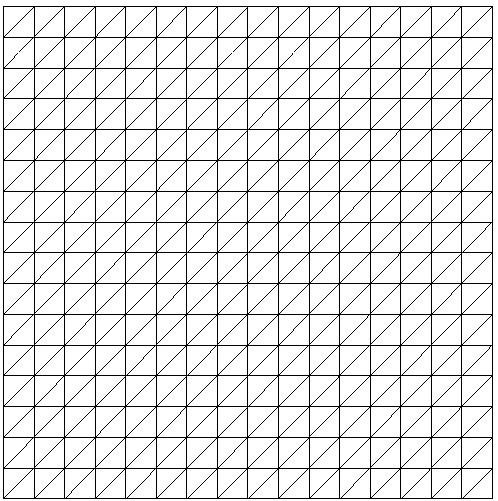
\includegraphics[width=0.15\textwidth]{figures/grid2.png}};
\node[roundnode] at (-3,9) (A){};
\node[above of=A]{\tiny \begin{tabular}{c}
  Input $x$\\\hline
  Initial Guess $u_0$\\ $r_0=f-A_1u_0$
\end{tabular}};
\node[roundnode] at (-4,9) (B){};
\node[left=1mm of B]{\tiny \begin{tabular}{c}
  $f^1 =F^1(x)$\\\hline
%$v_1=u_0+S_1r_0$\\
%$ r_1=f-A_1v_1$
$r_1 = F_1(r^0)$
\end{tabular} };
\node[inner sep=0pt] at (-10, 6){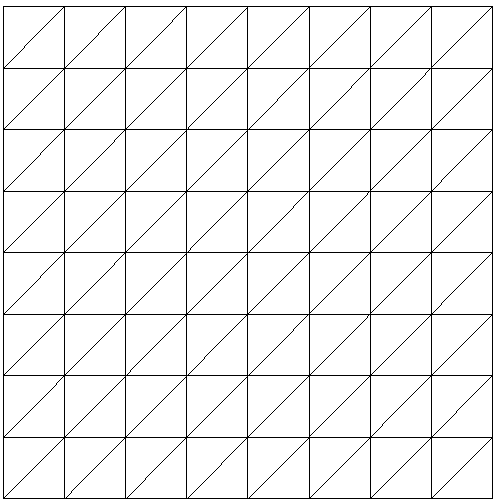
\includegraphics[width=0.15\textwidth]{figures/grid1.png}};
\node[roundnode] at (-3,6)  (C){};
\node[left=1mm of C]{\tiny \begin{tabular}{c}
$f^2=F^2(R_1^2f^1)$ \\\hline
%$v_2=S_2R_1^2r_1$\\ $r_2= R_1^2r_1-A_2v_2$
$r_2 = F_2(R^2_1r_1)$
\end{tabular} };
\node[inner sep=0pt] at (-10, 3){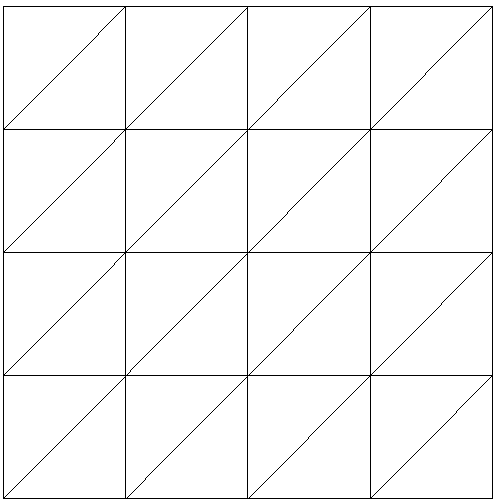
\includegraphics[width=0.15\textwidth]{figures/grid0.png}};
\node[roundnode] at (-2,3)  (D){};
\node[left=1mm of D]{\tiny \begin{tabular}{c}
$f^3=F^3(R_2^3f^2)$ \\\hline
%$v_3=S_3R_2^3r_2$\\ $r_3= R_2^3r_2-A_3v_3$
$r_3 = F_3(R^3_2r_2)$
\end{tabular} };
\node[inner sep=0pt] at (-10, 0){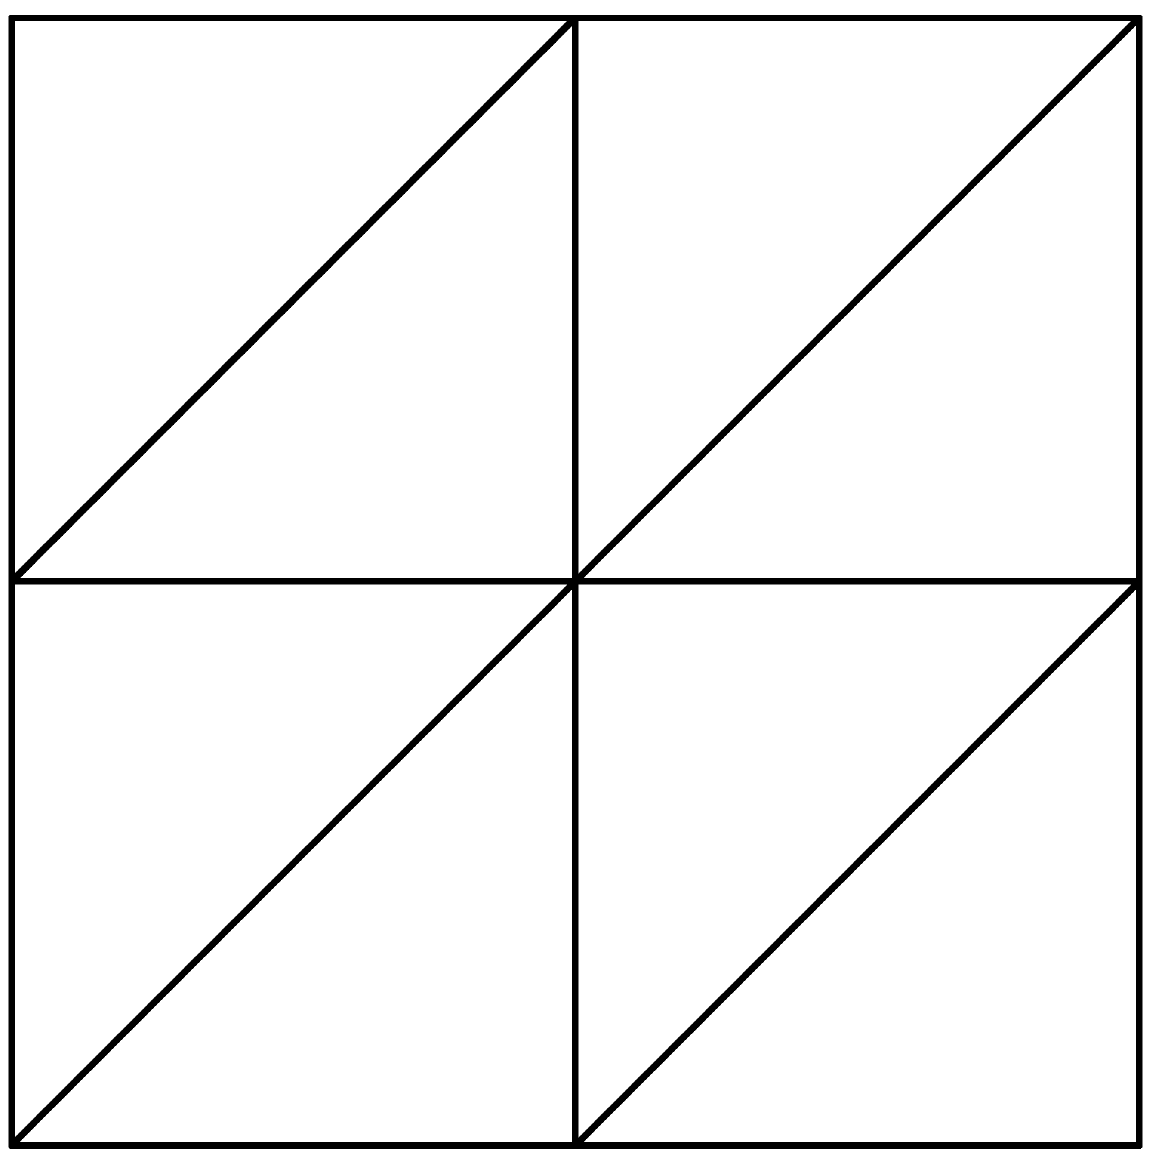
\includegraphics[width=0.15\textwidth]{figures/grid.png}};
\node[roundnode] at (-1,0)  (E){};
\node[below of=E]{\tiny \begin{tabular}{c}
$g^4=f^4=F^4(R_3^4f^3)$ \\\hline
$v_4= r_4 = F_4(R_3^4r_3)$
\end{tabular} };
\node[roundnode] at (0,3)  (F){};
\node[right=1mm of F]{\tiny \begin{tabular}{c}
$g^3 = G^3(P_4^3g^4)$  \\\hline
%$v_3\leftarrow v_3+(R_3^4)^Tv_4$ \\ $r_3=S_3(R_2^3r_2-A_3v_3)$\\ $v_3\leftarrow v_3+r_3$
$v_3 = G_3(P^3_4v_4)$
\end{tabular} };
\node[roundnode] at (1,6)  (G){};
\node[right=1mm of G]{\tiny \begin{tabular}{c}
$g^2 = G^2(P_3^2g^3)$  \\\hline
%$v_2\leftarrow v_2+(R_2^3)^Tv_3$ \\ $r_2=S_2(R_1^2r_1-A_2v_2)$\\ $v_2\leftarrow v_2+r_2$
$v_2 = G_2(P^2_3v_3)$
\end{tabular} };
\node[roundnode] at (2,9)  (H){};
\node[right=1mm of H]{\tiny \begin{tabular}{c}
$g^1 = G^1(P_2^1g^2)$  \\\hline
%$v_1\leftarrow v_1+(R_1^2)^Tv_2$ \\ $r_1=S_1(f-A_1v_1)$\\ $v_1\leftarrow v_1+r_1$
$v_1 = G_2(P^1_2v_2)$
\end{tabular} };
\node[roundnode] at (1,9)  (I){};
\node[above of=I]{\tiny \begin{tabular}{c}
  Output $y=ResNet(x)$\\\hline
  Solution $u\leftarrow u_0+B_\vee r_0$
\end{tabular}};
% lines
\draw[ultra thick, ->] (A)--(B) node[pos=.5,above,sloped] (TextNode) {};
\draw[ultra thick, ->] (B)--(C) node[pos=.5,above,sloped] (TextNode){};
\draw[ultra thick, ->] (C)--(D) node[pos=.5,above,sloped] (TextNode){};
\draw[ultra thick, ->] (D)--(E) node[pos=.5,above,sloped] (TextNode){};
\draw[ultra thick, ->] (E)--(F) node[pos=.5,above,sloped] (TextNode){};
\draw[ultra thick, ->] (F)--(G) node[pos=.5,above,sloped] (TextNode){};
\draw[ultra thick, ->] (G)--(H) node[pos=.5,above,sloped] (TextNode){};
\draw[ultra thick, ->] (H)--(I) node[pos=.5,above,sloped] (TextNode){};
\end{tikzpicture} }
\caption{Left: a nested multilevel grids; Right: a ${\rm V}$-cycle multigrid method 
	%(see \eqref{multi-backslash}-\eqref{eq:slash}) 
	versus a CNN model for segmentation 
  %(see  \eqref{multi-encode}-\eqref{multi-decode}) 
  .}
\label{fig:V-cycle}
\end{center}
\end{figure}


We consider a continuous linear finite element discretization of
\eqref{laplace} on a nested sequence of grids of sizes $n_\ell\times
n_\ell$ with $n_{\ell-1}=(n_\ell-1)/2$, as shown in the left part of
Fig. \ref{fig:V-cycle} and the corresponding sequence of finite
element spaces:
$$
V_1\supset V_2\supset\cdots\supset V_J.
$$
The discretized system is
\begin{equation}
\label{laplace-h}
Au=f.
\end{equation}
In correspondence with the two-dimensional grid, here we treat $f\in \mathbb R^{n\times n}$.  We need to find $u\in \mathbb R^{n\times n}$ satisfying \eqref{laplace-h}.
Here,  $A:\mathbb R^{n\times n}\mapsto \mathbb R^{n\times n}$ is a tensor satisfying
\begin{equation}
\label{uniform-laplace}
(Au)_{i,j}=4u_{i,j}-u_{i+1,j}-u_{i-1,j}-u_{i,j+1}-u_{i,j-1},
\end{equation}
which holds for $1\le i,j \le n$ whereas a slightly different formula holds for
other $i, j$. Here we notice that, there exist a $3\times 3$ kernel as
\begin{equation}\label{eq:kernel-A}
K_A = \begin{pmatrix}
0 & -1 & 0 \\
-1 & 4 & -1 \\
0 & -1 & 0
\end{pmatrix},
\end{equation}
with 
$$
Au = K_A \ast u.
$$
Where $\ast$ is the stander convolution operation with zero padding like \cite{goodfellow2017deep}. 
We now briefly describe a two-level multigrid method by
a mixed use of the terminologies from deep learning \cite{goodfellow2017deep} and multigrid methods.

The first main ingredient in GMG is a smoother.  A commonly used smoother is a
damped Jacobi,  which can be written as $S:\mathbb R^{n\times n}\mapsto
\mathbb R^{n\times n}$ satisfying
\begin{equation}
\label{jacobi1}
(Sf)_{i,j}={\omega\over 4}f_{i,j}.
\end{equation}
If we apply the Jacobian iteration twice, then
\begin{equation}
\label{jacobi2}
(S^2f)_{i,j}
={1\over 4}\omega(2-\omega)f_{i,j}+{\omega^2\over 16}(f_{i+1,j}+f_{i-1,j}+f_{i,j+1}+f_{i,j-1}).
\end{equation}
Then we have 
\begin{equation}\label{eq:kernel-S}
K_S = {\omega \over 4},
\end{equation}
and 
\begin{equation}\label{eq:kernel-S2}
K_{S^2} = \begin{pmatrix}
0 & \frac{\omega^2}{16} & 0 \\
\frac{\omega^2}{16} & {\omega(2-\omega) \over 4} & \frac{\omega^2}{16}  \\
0 & \frac{\omega^2}{16}  & 0
\end{pmatrix}
\end{equation}
Another ingredient is the restriction matrix $R: \mathbb R^{n_1\times
	n_1}\mapsto \mathbb R^{n_2\times n_2}$, which can be obtained by two
different steps. First, we carry out a convolution operation $\tilde
R: \mathbb R^{n_1\times n_1}\mapsto \mathbb R^{n_1\times n_1}$:
\begin{equation}
\label{linear-restriction}
(\tilde Rr)_{i,j}=r_{i,j}+{1\over 2}(r_{i-1,j}+r_{i+1,j}+r_{i,j-1}+r_{i,j+1}+r_{i-1,j-1}+r_{i+1,j+1}),
\end{equation}
Then, we define
\begin{equation}
\label{linear-restriction-stride}
(Rr)_{i,j}=(\tilde R r)_{2i-1,2j-1}, \quad 1\le i, j \le n_2.
\end{equation}
Using the terminology from deep learning \cite{goodfellow2017deep}, 
we note that \eqref{linear-restriction} can be written as a
convolution with a $3\times3$ kernel:
\begin{equation}
\label{convolution}
\tilde Rr=K*r,\quad K=\left ( \begin{array}{ccc}
0 &\frac{1}{2}&\frac{1}{2}\\
\frac{1}{2}& 1&\frac{1}{2}\\
\frac{1}{2}&\frac{1}{2}& 0
\end{array}\right ).
\end{equation}
Similarly, \eqref{jacobi1} is a convolution with a $1\times1$ kernel, 
\eqref{jacobi2} is a convolution with a $3\times 3$ kernel, and
\eqref{linear-restriction} and \eqref{linear-restriction-stride} is a
convolution with a stride. 

In general, we have restriction $R_{\ell-1}^\ell:\mathbb
R^{n_{\ell-1}\times n_{\ell-1}}\mapsto R^{n_{\ell}\times n_{\ell}}$ on
level $\ell$, and the corresponding prolongation is given by
$P_\ell^{\ell-1}=[R_{\ell-1}^\ell]^T$.  This restriction gives rise
to a restriction of $A=A_1$ on the coarse mesh:
$A_\ell=R_{\ell-1}^\ell A_{\ell-1}P_\ell^{\ell-1}: \mathbb
R^{n_\ell\times n_\ell}\mapsto \mathbb R^{n_\ell\times n_\ell}$
($\ell=2:J$).

Using the smoother $S$ and restriction $R$ above, a two-level
multigrid method for solving \eqref{laplace-h} can be written as
$u\leftarrow u_0, r\leftarrow f-Au$:
\begin{equation}
\label{2level}
u\leftarrow u+ Sr, \quad r\leftarrow f-Au, \quad u\leftarrow u+ B_2Rr,
\quad r\leftarrow f-Au, \quad u\leftarrow u+S R^Tr.
\end{equation}
In a two-level setting, we can take $B_2=A_2^{-1}$, or we can apply
\eqref{2level} recursively to obtain a multilevel V-cycle.     More
specifically, given $u_0\in V$,  this multilevel V-cycle can be
described as follows

From the fine to the coarse level, 
\begin{equation}\label{multi-backslash}
r_\ell = F_\ell (R^\ell_{\ell - 1} r_{\ell-1}), \quad 
w_\ell =[(I+S_{\ell}(I - A_{\ell} )]R^{\ell}_{\ell-1} r_{\ell-1}\quad \ell = 2:J,
\end{equation}
where
\begin{equation}\label{eq:backslash}
F_\ell (x) = x - A_\ell S_\ell x, \quad \ell = 1:J-1
\end{equation}
with 
$$
r_0=f-Au_0, r_1 = F_1(r_0),  F_J(x) = A_J^{-1}x.
$$ 
From the coarse to the fine level, 
\begin{equation}\label{multi-slash}
v_{\ell-1} = G_{\ell-1} (P^{\ell-1}_{\ell} v_{\ell}), \quad \ell = J:2,
\end{equation}
where
\begin{equation}\label{eq:slash}
G_{\ell-1} (x) = w_{\ell-1} + x - S_\ell A_\ell x
\end{equation}
with
$$
v_J = r_J = F_J(R^J_{J-1} r_{J-1}).
$$ 
An example of a $4$-level ($J=4$) V-cycle is illustrated in
Fig. \ref{fig:V-cycle}.

In a more general setting, \eqref{laplace-h} can be a general linear
algebraic system, with a slight abuse of notation here, such that
$u\in \mathbb R^N$ and $A: \mathbb R^N\mapsto \mathbb R^N$.  (In the
uniform grid case $N=n^2$.)  In this case, the AMG method can still be
written as in \eqref{2level}, but the smoother and restriction
matrices must be designed to maximize the algorithm efficiency.  In
multigrid methods, we almost always choose the prolongation
$P=R^T$. Thus the design of restriction is the same as the design of
prolongation.  Most of the existing AMG literature focuses on
designing an appropriate prolongation for a given smoother such as the
Jacobi iterative method.  In this proposal, we advance the field by
also considering the design of an appropriate smoother for a given
restriction.





\section{Convolutional neural networks}\label{sc:cnn}
Convolutional neural network, first introduced by LeCun
\cite{lecun1998gradient}, has been successfully applied to many
problems.  One of the most successful applications is for image
classification
\cite{lecun1998gradient,krizhevsky2012imagenet,simonyan2014very,he2016deep}.
Here,  for simplicity of exposition, we introduce CNN for image
de-noising
\cite{NIPS2008_3506,bengio2013generalized,alain2014regularized,xie2012image,zhang2017beyond}.
We emphasize that our introduction may not follow the standard
notation or terminology used in the deep learning literature. Instead
we borrow some notation and terminology from multigrid methods
for our descriptions.

Given an image $x \in \mathbb{R}^{n\times n}$ stained with 
noise (often assumed to be Gaussian), our goal is to use a deep neural
network to find a de-noised image such that $ y=f(x, \Theta) $.  The
function $f$, which depends on a set of parameters $\Theta$ and can be
viewed as a vector in $\mathbb R^{\mathcal N}$, will be given
in terms of a convolutional neural network  briefly described
next.  The parameter $\Theta$ can be obtained, for example, by
solving the following least squares problem:
\begin{equation}  \label{min-LSQ}
\min_{\Theta\in\mathbb R^{\mathcal N}}\mathcal L(\Theta), \quad
\mathcal L(\Theta)={1\over N}\sum_{i=1}^N \mathcal L_i(\Theta),
\quad \mathcal L_i(\Theta)=
\|f(x_i,\Theta)-\bar x_i)\|_{F}^2.
\end{equation}
Here, $x_i \in \mathbb{R}^{n\times n}$ ($i=1:N$), often referred to as training
data, are images obtained by adding noise to the corresponding
``clean'' images $\bar x_i$.

An image can be viewed as a function defined on a uniform grid.  We
assume that this uniform grid can be coarsened in a uniform fashion,
as shown in Fig. \ref{fig:V-cycle}.  As in multigrid methods, we
designate these grids as multilevel.  Every grid
represents a different level.  This is in contrast with the concept of
``layers'' in CNN in the deep learning literature
\cite{goodfellow2017deep}.  In Fig. \ref{fig:V-cycle}, the number of
levels is $J=4$. A CNN involves operations among different levels of
grids together with layers of nonlinear operations within each level
of grid.

A key ingredient of an artificial neural network is the 
activation function, which is always nonlinear.  A commonly used
activation function is ReLU defined as
\begin{equation}
\label{ReLU}
\sigma(t)=\max(0,t).
\end{equation}

\subsection{Operations from level to level}\label{ssc:level}
Given an image $x$, we first consider operations from fine to coarse
levels as follows:
\begin{itemize}
	\item Classical CNN model
\begin{equation}\label{multi-encode-classic}
f^{\ell} = F^{\ell}(R^{\ell}_{\ell -1} f^{\ell-1}), \quad \ell=2:J,
\end{equation}
	\item ResNet model
\begin{equation}\label{multi-encode}
f^{\ell} = R^{\ell}_{\ell -1} f^{\ell-1} + F^{\ell}(R^{\ell}_{\ell -1} f^{\ell-1}), \quad \ell=2:J,
\end{equation}
\end{itemize}
with $f^1 = F^1(x)$, $R^{\ell}_{\ell-1}: \mathbb R^{\hat
	c_{\ell-1}\times n_{\ell-1}\times n_{\ell-1}}\mapsto \mathbb
R^{c_\ell \times n_{\ell}\times n_{\ell}}$ is a restriction often
given by convolution with stride (or by pooling), and $F^\ell: \mathbb
R^{c_\ell \times n_{\ell}\times n_{\ell}}\mapsto \mathbb R^{\hat
	c_\ell \times n_{\ell}\times n_{\ell}}$ consists of a sequence of
convolution and nonlinear activation operations. \eqref{multi-encode}
is often referred as an encoding process by convolution.

Operations from coarse to fine levels can be defined similarly:
\begin{itemize}
	\item Classical CNN model
	\begin{equation}\label{multi-decode-classic}
	g^{\ell-1} = G^{\ell-1}(P^{\ell-1}_{\ell}g^{\ell}), \quad \ell=J:2,
	\end{equation}
	\item ResNet model
	\begin{equation}\label{multi-decode}
	g^{\ell-1} =P^{\ell-1}_{\ell}g^{\ell} + G^{\ell-1}(P^{\ell-1}_{\ell}g^{\ell}), \quad \ell=J:2,
	\end{equation}
\end{itemize}
with $g^{J} = f^J$.  Here, $P^{\ell-1}_{\ell}: \mathbb R^{c_{\ell}
	\times n_{\ell}\times n_{\ell}}\mapsto R^{\hat n_{\ell-1}\times
	n_{\ell-1}\times n_{\ell-1}}$ is a prolongation matrix of the same
size as the transpose of $R^{\ell}_{\ell-1}$ in \eqref{multi-encode}.
$G^{\ell-1}$ consists of a sequence of de-convolution and nonlinear
activations.  Further,  \eqref{multi-decode} is often known as a decoding
process by de-convolution.

\subsection{Multilayer operations within a given  level}\label{ssc:layer}

\subsubsection{Classical CNN model.}
For general CNN case, the $F^\ell$ and $G^\ell$ are defined for general CNN structure as: $F^\ell (y^{\ell,0}) = y^{\ell, m_\ell}$ with 
\begin{equation}\label{eq:gcnnblock}
y^{\ell, j} = \sigma \circ \theta^{\ell,j}(y^{\ell,j-1}),
\quad j = 1:m_\ell,
\end{equation}
where $y^{\ell,0} =R^{\ell}_{\ell-1} f^{\ell-1}$. We can have a similar formula for $G^j$ as $y^{\ell,0} =
P^{\ell}_{\ell+1} g^{\ell+1}$.
Here,  one key point is that $\theta^{\ell,j}$
are convolutional operations in the following form:
\begin{equation}\label{eq:conv-1}
[\theta^{\ell,j}(y)]_{i} = \sum_k^{c^{\ell,j-1}}K^{\ell, j}_{i,k} \ast y_k + b^{\ell,j}_i \bm{1} \in \mathbb{R}^{n_\ell \times n_\ell}, \quad i = 1:c_{\ell,j},
\end{equation}
where $\ast$ denotes the standard convolution operation (see
\eqref{linear-restriction} and \eqref{convolution} for example), and
$c^{\ell,j}$ denotes the number of channels or multiple smoothed
(coarse) spaces in the $j$-th layer in level $\ell$.

\subsubsection{New ResNet model.}
We now describe a special CNN model using a special form of ResNet
developed in \cite{he2016deep,he2016identity};  that is,  we need to
specify how $F^\ell$ and $G^\ell$ are defined.  Specifically, we can
define $F^\ell (y^{\ell,0}) = y^{\ell, m_\ell} -  y^{\ell, 0}$, with
$y^{\ell,0} =R^{\ell}_{\ell-1} f^{\ell-1}$ and, 
\begin{equation}\label{eq:resblock}
y^{\ell, j} = y^{\ell, j-1} + \mathcal{F}^{\ell, j}(y^{\ell,j-1}),
\quad j = 1:m_\ell.
\end{equation}
Here
\begin{equation}\label{eq:basic}
\mathcal{F}^{\ell,j}(y) = \xi^{\ell,j} \circ \sigma \circ \eta^{\ell,j}(y),
\end{equation}
as $\xi^{\ell,j}$ and $\eta^{\ell,j}$ are both general convolutions
with multi-channels. There are two observations for the basic structure \eqref{eq:basic}:
\begin{itemize}
	\item $ \xi \circ \sigma \circ \eta$ have the universal approximation for any continuous functions in compact sets for general fully connected deep neural networks.
	\item In the V-cycle method, especially for \eqref{eq:backslash} it is exact the case for \eqref{multi-encode} with $j=1$ for \eqref{eq:resblock}.
\end{itemize}


The same as general CNN models, we can have a similar formula for $G^j$ as $y^{\ell,0} =
P^{\ell}_{\ell+1} g^{\ell+1}$. This shows that, for this kind of model, we do residual for between both levels and layers as:
\medskip
\begin{table}[!htbp]
	\centering
	\footnotesize
	\begin{tabular}{|c|c|c|}
		\hline
		&level to level & layer to layer  \\
		\hline
		Iterative Formula  & $f^{\ell} = R^{\ell}_{\ell -1} f^{\ell-1} + F^{\ell}(R^{\ell}_{\ell -1} f^{\ell-1})$ & $y^{\ell, j} = y^{\ell, j-1} + \mathcal{F}^{\ell, j}(y^{\ell,j-1})$\\
%		\hline
%		Residual Form	 & $ F^{\ell}$ &$y^{\ell,1} = \mathcal{F}^{\ell, 1}(y^{\ell,0})$ \\
%		\hline
%		feature extractors &smoother (designed a priori) & convolution (trained) \\
%		\hline
%		grid transfer & restriction (designed a priori) & convolution with stride  (trained) \newline or pooling (given)\\
		\hline
	\end{tabular}
	\caption{\footnotesize A brief comparison between levels and layers.}
	\label{Level-Layes}
\end{table}

%So, now all the parameter as collected as
%\begin{equation}\label{para-level}
%	\Theta = \{\theta^1, \cdots, \theta^J, \theta^J, \theta^1\},
%\end{equation}
%as
%\begin{equation}\label{para-layer}
%	\theta^\ell = \{\eta^{\ell,0}, \xi^{\ell,0}, \cdots, \eta^{\ell,m_\ell}, \xi^{\ell,m_\ell}\}.
%\end{equation}

In comparing \eqref{multi-encode}-\eqref{multi-decode} for CNN with
\eqref{multi-backslash}-\eqref{eq:slash} for MG and the convolutions
\eqref{eq:conv-1} for CNN with the smoother \eqref{convolution} for
MG, we note that the CNN model described above is strikingly similar
to the structure of the V-cycle multigrid method as illustrated by
Fig.~\ref{fig:V-cycle}.


In our terminology, the number of layers in deep learning literature
is associated with the total number of applications of the activation
and is equal to $\sum_{\ell=1}^Jm_\ell$.  Within a given level, the
number of layers can be compared with the number of smoothings used in
multigrid methods.



%CNN used for purpose of de-noising has been studied extensively in the
%literature, including in
%\cite{NIPS2008_3506,bengio2013generalized,alain2014regularized,xie2012image,zhang2017beyond}.
%We also have performed some experiments of this kind by adding
%Gaussian noise to a MNIST dataset and then using the aforementioned CNN
%procedure for de-noising.  The results are remarkably good as observed
%in many existing studies referenced above, and,  as shown in
%Fig.~\ref{noise-denoise} in which the bottom images are the de-noised
%images of the ones above.

\section{Connections between multigrid method and CNN}
We now offer a comparison between geometric multigrid methods (GMG)
and convolutional neural networks (CNN).  It is this comparison
between these two distinctive methodologies that motivates much of the
research described in this proposal.  A brief summary of our comparison is
given in Table~\ref{MG-CNN}.
\medskip
\begin{table}[!htbp]
	\centering
	\footnotesize
	\begin{tabular}{|l|l|p{40mm}|c|}
		\hline
		&Multigrid &CNN  \\
		\hline
		goals  & linear system solver & image denoising or classification \\
		\hline
		structure	 &multilevel grids with multiple smoothings &multilevel grids with multiple convolutions and activations \\
		\hline
		feature extractors &smoother (designed a priori) & convolution (trained) \\
		\hline
		grid transfer & restriction (designed a priori) & convolution with stride  (trained) \newline or pooling (given)\\
		\hline
	\end{tabular}
	\caption{\footnotesize A brief comparison between MG and CNN.}
	\label{MG-CNN}
\end{table}

First we note that MG and CNN are both based on a hierarchy level of
``grids'' although the notion of a ``grid'' is not often discussed in
the CNN literature.   MG is a linear algorithm for solving linear system of equations
whereas CNN is a  nonlinear model designed for image de-noising or
classification.  On each level, MG uses a given method such as Jacobi or
Gauss-Seidel as a smoother, whereas CNN uses multiple ``channels'' of
convolutions.    The similarity here is that a smoother such as the damped
Jacobi can be interpreted as a convolution of the size $1\times 1$ or
$3\times 3$.  The difference between the two methods on this point is
that in MG the smoother is designed a priori
and usually only one smoother is used on each level, whereas in CNN,
the convolution is trained and multiple channels of convolutions are
used.   From fine to coarse (or vice-versa), restriction  matrices are used in both
methods, but again the difference remains: the restriction in MG is
designed a priori,  whereas in CNN the restriction is trained (as a
convolution with stride) or sometimes is given a priori (by an
operation called ``pooling'').

\subsection{V-cycle and U-net}
If we compare the V-cycle and new ResNet model, we may mention formula, 
U-net \cite{ronneberger2015u} structure likes the V-cycle very much. Here we will give more comparison on those two structures. 
%Let us show the U-net model with ResNet structure in mathematically. 
\subsubsection{Segmentation problem}
Here we introduce some basic background about segmentation problem.....
\subsubsection{Classical U-net model}
The U-net was proposed firstly in \cite{ronneberger2015u} based on the classical CNN model as introduced in \S \ref{sc:cnn}. A mathematical expression of this model is:
\begin{itemize}
	\item Encode phase
	\begin{equation}\label{U-multi-encode-classic}
	f^{\ell} = F^{\ell}(R^{\ell}_{\ell -1} f^{\ell-1}), \quad \ell=2:J,
	\end{equation}
	for $f^1 = F^1(x)$ and
	$F^\ell (y^{\ell,0}) = y^{\ell, m_\ell}$ with 
	\begin{equation}\label{u-eq:gcnnblock}
	y^{\ell, j} = \sigma \circ \theta^{\ell,j}(y^{\ell,j-1}),
	\quad j = 1:m_\ell,
	\end{equation}
	where $y^{\ell,0} =R^{\ell}_{\ell-1} f^{\ell-1}$.
	
	
	\item Decode phase
	\begin{equation}\label{U-multi-decode-classic}
	g^{\ell-1} = G^{\ell-1}([P^{\ell-1}_{\ell}g^{\ell},C^{\ell-1}f^{\ell-1}]), \quad \ell=J:2,
	\end{equation}
	for $g^{J} = f^J$ and $G^\ell (y^{\ell,0}) = y^{\ell, m_\ell}$ with 
	\begin{equation}\label{eq:gcnnblock}
	y^{\ell, j} = \sigma \circ \theta^{\ell,j}(y^{\ell,j-1}),
	\quad j = 1:m_\ell,
	\end{equation}
	where $y^{\ell,0} = [P^{\ell-1}_{\ell}g^{\ell},C^{\ell-1}f^{\ell-1}]$. Here $[P^{\ell-1}_{\ell}g^{\ell},C^{\ell-1}f^{\ell-1}]$ means to collect the prolongated result $P^{\ell-1}_{\ell}g^{\ell}$ and the rescale cut for $f^{\ell-1}$ (the dimension reduction for segmentation results) as a new image with double size channels(One comes form $f$ one comes form $g$). 
\end{itemize}


\subsubsection{Connections between V-cycle and U-net}
\begin{itemize}
	\item Structure of coarse and prolongation.
	\item Basic structure in universal approximation theory.
	\item PDE-based model expression.
\end{itemize}


\subsubsection{New U-net model motivated by V-cycle}
Now we proposed a new U-net model as:
\begin{itemize}
	\item Encode phase
	\begin{equation}\label{U-multi-encode}
	f^{\ell} = R^{\ell}_{\ell -1} f^{\ell-1} + F^{\ell}(R^{\ell}_{\ell -1} f^{\ell-1}), \quad \ell=2:J,
	\end{equation}
	for $f^1 = F^1(x)$. 
	$F^\ell (y^{\ell,0}) = y^{\ell, m_\ell} -  y^{\ell, 0}$, with
	$y^{\ell,0} =R^{\ell}_{\ell-1} f^{\ell-1}$ and, 
	\begin{equation}\label{u-eq:resblock}
	y^{\ell, j} = y^{\ell, j-1} + \mathcal{F}^{\ell, j}(y^{\ell,j-1}),
	\quad j = 1:m_\ell,
	\end{equation}
	for
	\begin{equation}\label{u-eq:basic-f}
	\mathcal{F}^{\ell,j}(y) = \xi^{\ell,j} \circ \sigma \circ \eta^{\ell,j}(y).
	\end{equation}
	
	\item Decode phase
	\begin{equation}\label{U-multi-decode}
	g^{\ell-1} = C^{\ell-1}f^{\ell-1} + P^{\ell-1}_{\ell}g^{\ell} + G^{\ell-1}(P^{\ell-1}_{\ell}g^{\ell}), \quad \ell=J:2,
	\end{equation}
	for $g^{J} = f^J$. 
	$G^{\ell-1} (y^{\ell-1,0}) = y^{\ell-1, m_{\ell-1}} - y^{\ell-1,0}$ with 
	$y^{\ell-1,0} = P^{\ell-1}_{\ell}g^{\ell}$
	\begin{equation}\label{u-eq:rcnnblock}
	y^{\ell-1, j} = y^{\ell-1, j-1} + \mathcal{G}^{\ell-1, j}(y^{\ell,j-1}),
	\quad j = 1:m_{\ell-1},
	\end{equation}
	for
	\begin{equation}\label{u-eq:basic-g}
	\mathcal{G}^{\ell-1,j}(y) = \phi^{\ell-1,j} \circ \sigma \circ \psi^{\ell-1,j}(y).
	\end{equation}
\end{itemize}


\section{Some general CNN structure motivated by V-cycle}
Here we will talk about more observations for V-cycle method writing as a ResNet model.
